\documentclass[12pt, a4paper, twoside]{book}
\usepackage{import}
\subimport{../}{preamble}
\begin{document}

\chapter{Introduction}

% Introduction to nanophotonics
Plasmonics is part of the greater field of nanophotonics - the understanding and application of light beyond the diffraction limit. Since light is limited in scale by the aforementioned diffraction limit, nanophotonics is instead dictated primarily by light-matter interactions. Under the influence of an incident electromagnetic wave, matter can become polarised resulting in the emission of radiation. The properties of the scattered field are then dictated by the physical characteristics of the matter. By this mechanism the optical properties of metals on the nm-scale become particularly interesting.
% Plasmons in general
Plasmonics is the name given to the study and application of plasmon quasiparticles - excitations of collective oscillations of free electrons {\color{red} in a metal}, to which the plasmon is the quantum. By transferring photon energy into free electron oscillations the photonic limits of optical confinement can be overcome.
% Plasmon coupling with light - surface plasmon polaritons
Under such conditions, light can be confined to sub-wavelength dimensions at the surface of the metal in the form of a surface charge oscillation - a surface plasmon.

% Properties of SPPs
Surface plasmons are charge density waves, evanescently confined to a metal-dielectric interface. They maintain the same frequency as their photonic excitation, however their wavelength is below the diffraction limit. This is the first interesting property of the plasmon. Secondly, as light becomes confined to a metallic surface in the form of a plasmon {\color{red}it retains its energy.} Charge accumulates at the surface, thus the electric field surrounding a strongly confined plasmon becomes strongly enhanced. This resonant near-field enhancement is the next most interesting property of a plasmon and the basis for nearly all applications of plasmonics to date.\footnote{The other main exploitation being the resonant position for refractive index sensing.}

% Localised surface plasmons
\begin{figure}[bt]
\centering
\fontsize{10pt}{1em}\selectfont
\def\svgwidth{0.6\textwidth}
\subimport{./figures/}{aunp_plasmon_diagram.pdf_tex}
\caption[Diagram of a localised surface plasmon in a AuNP.]{\textbf{Diagram of a localised surface plasmon in a AuNP.} Electrons move to screen the external field from the AuNP. The charge density at the electromagnetic poles of the surface greatly enhances the local field.}
\label{fig:aunp_plasmon}
\end{figure}

Noble metal nanoparticles have particularly good surface plasmons in the visible region of the electromagnetic spectrum, and are therefore used in the majority of all work involving plasmonics. Their electrons are highly mobile and freely move to oppose an incident field, leading to strong collective oscillations of conduction electrons. Their inertia, however, leads to this behaviour becoming resonant at specific frequencies. Light shining on a sub-wavelength, noble metallic nanoparticle can therefore readily couple with surface plasmon resonances that remain highly localised on the particle surface (\figurename~\ref{fig:aunp_plasmon}). A direct result of this is resonant evanescent enhancement of the incident field at the plasmon poles.

% Concept of an optical antenna
\begin{figure}[bt]
\centering
	\includegraphics[width=0.45\textwidth, clip=true, trim=0 650 0 0]{figures/literature/nphoton_2010_237_f1}
	\includegraphics[width=0.45\textwidth, clip=true, trim=15 0 0 660]{figures/literature/nphoton_2010_237_f1}\\
%\includegraphics[width=0.45\textwidth]{figures/literature/nphoton_2010_237_f3}
\caption[The concept of an optical nano-antenna \cite{novotny2011}.]{\textbf{The concept of an optical nano-antenna \cite{novotny2011}.} The electric field from a near-field transmitter is coupled via an antenna into far-field radiation. By reciprocity, far-field radiation can be received in the near-field. Plasmonic nanostructures act as optical antennae.}
\label{fig:novotny2011}
\end{figure}

As external (far-field) photonic fields readily couple with nanoparticles they have becomes known as optical antennae, in analogy with conventional metal radio wave antennae (\figurename~\ref{fig:novotny2011}). Consequently, they are seen as a simple and efficient method for transferring and confining photonic energy to nanoscale dimensions. Energy can then be transferred to nano-emitters, such as quantum dots, or even between plasmons in the form of an interaction field.
% Plasmon interactions
As a plasmon is simply a charge oscillation, similar in many cases to a {\color{red}point} dipole, it is susceptible to interactions with other dipoles. When two plasmons come into close proximity their modes interact, causing the resonant frequency of the coupled system to redshift, and the near-field becomes strongly confined to the space between plasmons. The smaller the space between dielectric and metallic surfaces the stronger the confinement of light into the dielectric. The result of this compression is a strong increase in the electric field stored within the region. Field strengths can readily increase up to $10^7$ times the incident photonic field. Such regions are known as 'hot spots' and form the basis for most plasmonic sensing platforms.

% SERS and SNOM - applying the field enhancement
Sensing has become the primary application of plasmonics since its inception. Applications of the plasmonic field enhancement have led to the development of now widely used techniques, such as surface-enhanced Raman scattering (SERS) \cite{fleischmann1974, jeanmaire1977} and scanning near-field optical microscopy (SNOM) \cite{}.
As with the plasmon and its resonant polarisability spectrally shaping the scattered field, the signature of molecular bonds is imprinted in the emitted radiation from optically polarised molecules due to inelastic scattering. This is the basic description of Raman scattering \cite{raman1928}. However, inelastic scattering from molecules is weak since the wavelength of light is order of magnitudes larger than the molecule, therefore the interaction cross-section is small. By coupling photons into plasmons the spatial field size difference becomes comparable and the interaction cross-section is greatly increased. By reciprocity electromagnetic fields in the near-field can be efficiently coupled into far-field photons via plasmons. This is the effect of the field enhancement. By placing molecules in the vicinity of a plasmonic surface and utilising the plasmonic field Raman scattering can be greatly enhanced by $\left|E/E_0\right|^4$. SNOM is similar in that electromagnetic scattering on the near-field is efficiently transmitted into the far-field. By further increasing the field enhancement in a plasmonic system it has become possible to even detect light scattering from just a few molecules within a single hot spot \cite{}.

% Introduction to sub-nm plasmon coupling and the quantum regime
\begin{figure}[bt]
\centering
\begin{tikzpicture}
\node[anchor=south west] at (-1.3,-1.5) {\includegraphics[width=0.9\textwidth]{data/plasmonic_regimes_background}};
\node[anchor=south west] at (0,0) {\includegraphics{data/plasmonic_regimes_foreground}};
\end{tikzpicture}
\caption[Regimes of plasmonic interaction.]{\textbf{Regimes of plasmonic interaction.} The diagram shows the coupling strength between two plasmonic particles across the full range of characteristic separation dimensions. At distances greater than the particle radius plasmons are uncoupled. Classical mode coupling begins at separations below the particle radius. Many nanoscale phenomena, such as capillary force/surface tension snap-in occur at these characteristic separations. Once the separation transitions to below \SI{1}{nm} quantum mechanical effects begin to become important. The quantum regime is the point at which these effects significantly effect plasmonic interaction.}
\label{fig:plasmonic_regimes}
\vspace{-10pt}
\end{figure}

If we are to push the boundaries towards single molecule plasmonic sensing, intuition suggests that plasmonic systems must become increasingly smaller to better confine light into 'hot spots' and further increase the localised near-field enhancement. Inevitably though, the characteristic dimensions of the nano-gaps forming the hot spots, or the particles themselves, becomes sufficiently small that quantum mechanical effects are no longer negligible (\figurename~\ref{fig:plasmonic_regimes}). Plasmonics on this sub-nm length scale currently has only a limited understanding. To a certain extent this has been due to difficulty fabricating structures that can enter this 'quantum regime'. Few reports have conclusively shown the influence of quantum effects on plasmonic performance.
It is therefore an interesting and relatively new and untouched topic that requires exploring.

% The correct measurements to understand the quantum regime
Ideally a difficult to access regime such as the quantum regime could be experimentally mapped in a manner similar to theory, using precisely positioned individual nanoparticles coming closer together. While there are methods for controlling nanoparticle positions further difficulty arises as to what measurements are then possible within that system. There exists a rich amount of fundamental physics occurring in sub-nm gaps that influences the plasmonic behaviour. To probe these effects requires sensitive measurements of charge transfer and forces not compatible with individual nanoparticle experiments. In order to experimentally access such a regime, we require precise nanopositioning of an electrically contacted nanoparticle with force sensitivity. For this reason, AFM probes become appealing devices as a means of controllably progressing into the sub-nm regime whilst simultaneously making the necessary measurements to understand the plasmonics. To enable this work the plasmonics of tips must be understood.

% The use of tips for plasmonics
Metallic tip structures at a glance are promising plasmonic probes as the characteristic dimensions of their apices fall well below the diffraction limit.
Furthermore, a clear advantage to using tips as plasmonic probes is the maturity of the many surface science techniques used for characterising nanoscale topology. Techniques such as scanning tunnelling microscopy (STM) \cite{binnig1982} and atomic force microscopy (AFM) \cite{binnig1986} have formed the foundation of surface analysis studies since their inception. The merging of tip-based topological scanning techniques with optical microscopy forms the basis of what has become known as tip-enhanced near-field optical microscopy (TENOM). The combination of toplogical, electronic, force and spectroscopic measurements enabled mapping of the nanoscale in more detail than previously possible, making TENOM a powerful tool for surface science. To date tips have shown great promise for sub-diffraction limited optical microscopy when utilised through such techniques. Despite this, the plasmonics of tips are still not yet fully understood.

\section{Project Outline}

The purpose of this project is twofold. It is firstly to demonstrate robust measurements of plasmonics in the sub-nm regime, from which a better understanding of the influence of quantum effects can de derived. By using a combined atomic force-optical microscope and two opposing, plasmonic tips the coupling between plasmons can be dynamically probed using multiple, simultaneous, correlated measurements from which we can ultimately understand the influence of quantum effects.
Two controllable AuNPs mounted onto conductive AFM tips are used to dynamically probe optical scattering from a plasmonic nano-gap whilst also measuring the conductance and the force. To achieve the desired robustness of measurements, the technology required to reliably produce dynamically controllable plasmonic nano-gaps is developed. This amounts to designing an experimental microscope capable of making the measurements and developing robust plasmonic tips.
The second aim of this project is to better understand the effect of tip geometry on its properties as an optical antenna. From this point the application of plasmonic tips in tip-based techniques can be explored.

% The outline of the chapters
This report begins with the necessary theoretical background to understand plasmons and plasmonic phenomena, discussing the types of plasmons and the coupling between them. The previous uses of tips for plasmonics, along with their current understanding, are then discussed. The experimental work is discussed in three parts: the production of plasmonic AFM tips by nanostructuring, the design and construction of a microscope capable of making stable measurements on an AFM tip dimer in the sub-nm regime, for use in the microscope, and finally the results of the experiments. The results are broken down into understanding the plasmonics of individual nanostructured tips and then understanding the coupling between two of them as their separation progresses into the sub-nm quantum regime.

\end{document}